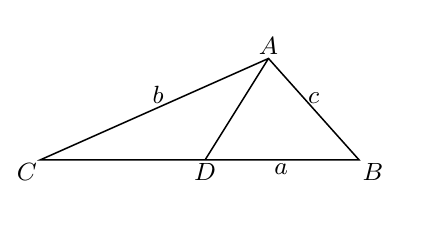
\begin{tikzpicture}[x=.023cm,y=-.023cm,baseline=(current bounding box.center),line width=.55pt,
  every node/.style={font=\small,inner sep=1pt}]
  \path[use as bounding box] (0,0) rectangle (204,103);
  \coordinate (C) at (7,73);
  \coordinate (D) at (98,73);
  \coordinate (B) at (183,73);
  \coordinate (A) at (133,17);
  \draw (C)--(A)--(B)--cycle (A)--(D);
  \node[below left] at (C) {$C$};
  \node[below] at (D) {$D$};
  \node[below right] at (B) {$B$};
  \node[above] at (A) {$A$};
  \node[above] at (72,44) {$b$};
  \node[above] at (158,44) {$c$};
  \node[below] at (140,73) {$a$};
\end{tikzpicture}
